% !TeX root = ../../msc-thesis.tex
\documentclass[../../msc-thesis.tex]{subfiles}

\begin{document}

\section{The $C_{4}$ Isomerization Process}

The last case-study presented consists in a $C_{4}$ isomerization process, 
that aims to convert \textit{n}-butane($n-C_{4}$) into isobutane ($i-C_{4}$). 
The latter can be used as an octane-enhancing gasoline blending agent, and 
also it is an precursor for isobutyl alcohol production 
\textcite{Jagtap2012}. The process described in this case-study it is based 
on the work of \cite{Jagtap2012}: Base operating conditions and optimal 
operating ones. The idea of this case study is to depict to reader the second
mode of operation that can be used in \mtc, described in 
\Cref{subsection:mtcworkflow} when the optimal operating point it is known. 
This was implemented within \mtc because there is a plethora of papers and 
discussions over the several years that addresses the optimization of several
processes (\cite{Jagtap2012,Jagtap2013,Araujo2007,Araujo2008,Gera2013,Liu2019,
Skogestad2004}, just to name a few), and when one is dealing with economic 
plantwide control specially, there are several results that can be anticipated 
regarding active constraints. For a deeper understanding, the reader should 
refer to \Cref{section:discussion}, \Cref{subsection:point2}. 

Thus, it is understood that there is a relevant number of experienced 
researchers that have interest in using the the local methods derived by 
\textcite{Halvorsen2003,Alstad2009} in order to find self-optimizing variables 
(or linear combinations of measurements), but already know constraints that 
must be controlled on their particular applications, specially when this task 
can be done in a comprehensive software environment, which is the case for
\mtc. In such cases, there is no need to used mode 1 from \mtc, and the user 
can simply build a metamodel of the reduced-space problem, merely providing 
the simulation file of the process with the active constraints already 
implemented, and sample the process using the unconstrained degrees of 
freedom, in order to generate the necessary high-order data, to finally 
obtain the most promising CV candidates.

The process flowsheet can be found on figure \ref{fig:c4processflowsheet}. 
The process was already optimized by \textcite{Jagtap2012} as stated before. 
Therefore, the authors used the previously found optimal point from the 
aforementioned work, and it is described in \Cref{tab:c4optpoint}. For this 
process, \textcite{Jagtap2012} kept the composition of \textit{n}-butane on 
the bottoms of the purge column constant, and the other variables that are 
fixed were active constraints of the optimization problem: Either anticipated 
or calculated, except regarding the cooler temperature, that was alleged to 
have little impact on the objective function, and it was kept constant. 
Therefore, the aforementioned fixed composition will be considered as an 
unconstrained degree of freedom, differently from \textcite{Jagtap2012}, 
and the reason is to evaluate if there is another variable that is easier 
to control than a composition that can be used in the control structure.

\begin{figure}[htb]
    \centering
    \caption{C4 Isomerization process flowsheet.}
    \label{fig:c4processflowsheet}
    \makebox[1.0\textwidth]{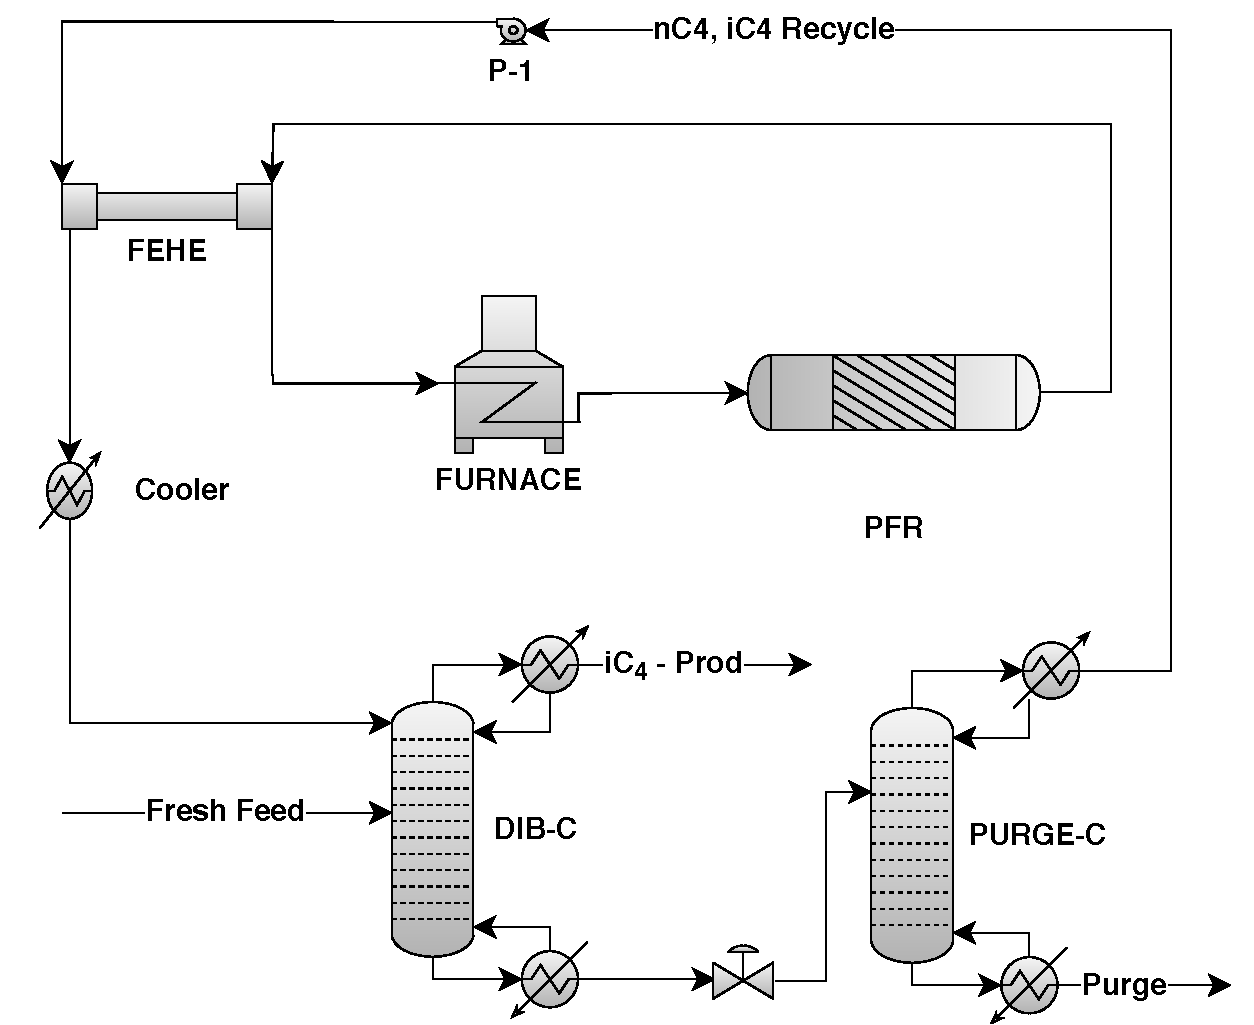
\includegraphics[width=1.0\textwidth]
    {c4isoflowsheet.pdf}}
\end{figure}


\begin{table}[htb]
    \centering
    \caption{C4 Isomerization process optimization summary.}
    \begin{tabular}{lll} \hline
        Objective Function: Profit [$\$/h$]  \\
        $ J = - 9.83 \times Q_{furnace} - 4.83\times(Q^{reboiler}_{DIB-C}+Q^{reboiler}_{PURGE-C}) $\\ 
        $- 0.16\times (Q^{condenser}_{DIB-C} + Q^{condenser}_{PURGE-C})$ \\ 
        $- 32.5\times F_{C_4} + 42\times F_{i-C_4} + 22\times F_{i-C_5}$\\ \hline
        Process constraints& \\
        $T_{\mathrm{reactor}}=200^{\circ} \mathrm{C}$ (active) & $0 \leq Q_{\text {furnace }} \leq 1.3$ (base-case) \\
        $0 \leq V_{1} \leq 1.3$ (base-case)       & $P_{\mathrm{reactor}}=45$ bar (active) \\
        $0 \leq V_{2} \leq 1.5$ (base-case)        & \\
        $T_{\mathrm{cooler}}=53^{\circ} \mathrm{C}$ (fixed)\\ \hline
        Unconstrained degrees of freedom\\
        $x_{i-C_{4}}^{B1} = 0.0565 $ & $x_{i-C_{5}}^{D2} = 0.02 $ \\
        $x_{n-C_{4}}^{B2} = 0.01 $\\ \hline
    \end{tabular}
    \label{tab:c4optpoint}
\end{table}

In \Cref{fig:c4mainscreen}, it can be seen that the only expression 
built for this problem was the economic objective function, due to the fact 
that the problem is already unconstrained (the active constraints are already 
known). Similarly to the first and second case studies, the user must 
identify the process disturbances, CV candidates and degrees of freedom 
(\Cref{fig:c4variables}).

\begin{figure}[htb]
    \centering
    \caption{C4 Isomerization process - loading simulation. The cooling water 
    price is positive due to signal convention inside the process simulator - 
    heat removed from the system has a negative sign.}
    \label{fig:c4mainscreen}
    \makebox[1.0\textwidth]{\includegraphics[width=1.0\textwidth]
    {c4mainscreen.PNG}}
\end{figure}


\begin{figure}[htb]
    \centering
    \caption{C4 Isomerization process - loading variables.}
    \label{fig:c4variables}
    \makebox[1.0\textwidth]{\includegraphics[width=1.0\textwidth]
    {c4-loadvar.PNG}}
\end{figure}

For the expected disturbances, the values come from \textcite{Jagtap2012}, 
and disturbances for the amounts of isobutane and \textit{n}-butane in the 
feed were considered, with a range of $10\%$ of the nominal values. 
However, instead of considering the compositions, the values of the 
individual component flow rates were used in the design of experiments. 
Regarding CV candidates, sensitive temperatures at the optimal operating 
point were inspected for both columns, and the most sensitive ones were 
considered as CV candidates. The full list of CV candidates can be seen 
in \Cref{tab:c4cvs}.

\begin{table}[htb]
    \centering
    \caption{CV Candidates for $C_{4}$ Isomerization process.}
    \begin{tabular}{l l}
    \hline
    \textbf{Variable} (alias used in \mtc) & \textbf{Description} \\ \hline
    c1\_t``x'     & 1st column stage X temperature (stages 21-33) $(\celsius)$ \\
    c2\_t``x'     & 2nd column stage X temperature (stages 14-20) $(\celsius)$ \\
    x\_ic4\_b1     & 1st column $i-C_{4}$ bottoms composition\\
    x\_ic5\_d2     & 2nd column $i-C_{5}$ distillate composition \\
    x\_nc4\_b2     & 2nd column $n-C_{4}$ bottoms composition\\
    c1\_v         & 1st column boilup rate $(kmol/h)$\\
    c2\_v         & 2st column boilup rate $(kmol/h)$\\
    c1\_l         & 1st column reflux rate $(kmol/h)$\\
    c1\_l         & 2nd column reflux rate $(kmol/h)$\\
    \hline
    \end{tabular}
    \label{tab:c4cvs}
\end{table}

50 points were sampled with an amplitude of $\pm0.5\%$ around the optimal 
point (\Cref{fig:c4redspace}), and the gradients and hessians could be 
extracted (\Cref{fig:c4grad}). Lastly, Similarly as the previous cases, the 
implementation error for temperatures was considered as $0.5\celsius$,
$10^{-3}$ for flow rates and $10^{-6}$ for compositions. All the 
aforementioned data was inserted inside \mtc, as can be seen in 
\Cref{fig:c4soc}.

\begin{figure}[htb]
	\centering
	\caption{C4 Isomerization process - loading variables.}
	\label{fig:c4redspace}
    \makebox[1.0\textwidth]{\includegraphics[width=1.0\textwidth]
    {c4redspace.PNG}}
\end{figure}

\begin{figure}[htb]
	\centering
	\caption{C4 Isomerization process - High-order data obtainment.}
	\label{fig:c4grad}
    \makebox[1.0\textwidth]{\includegraphics[width=1.0\textwidth]
    {c4grads.PNG}}
\end{figure}

\begin{figure}[htb]
	\centering
	\caption{C4 Isomerization process - Self-Optimizing Control input.}
	\label{fig:c4soc}
    \makebox[1.0\textwidth]{\includegraphics[width=1.0\textwidth]
    {c4socinput.PNG}}
\end{figure}

For the sake of brevity only the single measurement policy was considered in 
this analysis. \Cref{fig:c4socresult} shows that, not surprisingly, the 
control of sensitive temperatures and the composition of the pollutant 
(in this case, $i-C_{5}$), yielded the lowest losses. However, keeping 
temperatures and flow rates with constant setpoints instead of using 
compositions are also promising control structures, as can be seen in 
\Cref{fig:c4socresult2}

\begin{figure}[htb]
	\centering
    \caption{C4 Isomerization process - Single measurements policy: Best 
    CV candidates.}
	\label{fig:c4socresult}
    \makebox[1.0\textwidth]{\includegraphics[width=1.0\textwidth]
    {c4-best-cvs.PNG}}
\end{figure}
	
\begin{figure}[htb]
	\centering
    \caption{C4 Isomerization process - Single measurements policy: Best 
    CV candidates not using compositions.}
	\label{fig:c4socresult2}
    \makebox[1.0\textwidth]{\includegraphics[width=1.0\textwidth]
    {c4-best-cvs-3.PNG}}
\end{figure}

\FloatBarrier

\end{document}